\appendix

\section{Appendices}

\subsection{Fréchet Web App}

The Fréchet web app and its development is not the focus of this paper; nevertheless, some background information about the visualisation software and the implementation of the algorithm may be useful.

\subsubsection{Development}

Initially, the algorithm without support for degenerate inputs was implemented in python as part of a software project.\

For the Bachelors thesis, I extended the algorithm towards supporting degenerate inputs by dealing with multiple critical events at same height $\epsilon_0$ using the traversability graph and the first derivative of the hyperbolas inverses.\

A web frontend was added to make visualising easy and intuitive.

\subsubsection{Live Version and Links}

The web app is accessible at \url{https://abegehr.github.io/frechet/}. While studying this paper, it is highly advised to use the links to the Fréchet web app to view examples that are appended throughout the text. The web app has features that make understanding examples easier that viewing a static picture.\

\subsubsection{Source Control}

The corresponding GitHub repository is reachable at \url{https://github.com/abegehr/frechet}. The GitHub repository hosts the current version of the source code, the commit history, as well as open and closed issues. It is also possible to fork the repository and edit the source code to add features and run a private version of the algorithm and the visualisation.

\subsubsection{Architecture}

The Fréchet web app consists of a python backend and a React frontend.\

A free Heroku dyno hosts the python backend. The backend API opens one endpoint that receives two input paths and returns the visualisation data. The API is reachable at \url{https://frechet-server.herokuapp.com}.\

The React frontend allows the user to input two paths consisting of straight line-segments, communicates with the python backend, and visualises the results computed by the python backend. GitHub static pages hosts the frontend.\

Initially, the \textit{Userpage} provided by the \textit{zedat} service of the \textit{Freie Universität Berlin} was to be used for hosting the whole Fréchet web app, but versioning problems and insufficient support made this unfeasible.

\subsubsection{Features}

To execute a run of the lexicographic Fréchet matchings algorithm, first visit the web app at \url{https://abegehr.github.io/frechet/}. Then continue as follows:

\begin{enumerate}
	\item Input two paths by clicking or by entering coordinates.
	
	\begin{figure}[H]
		\centering
		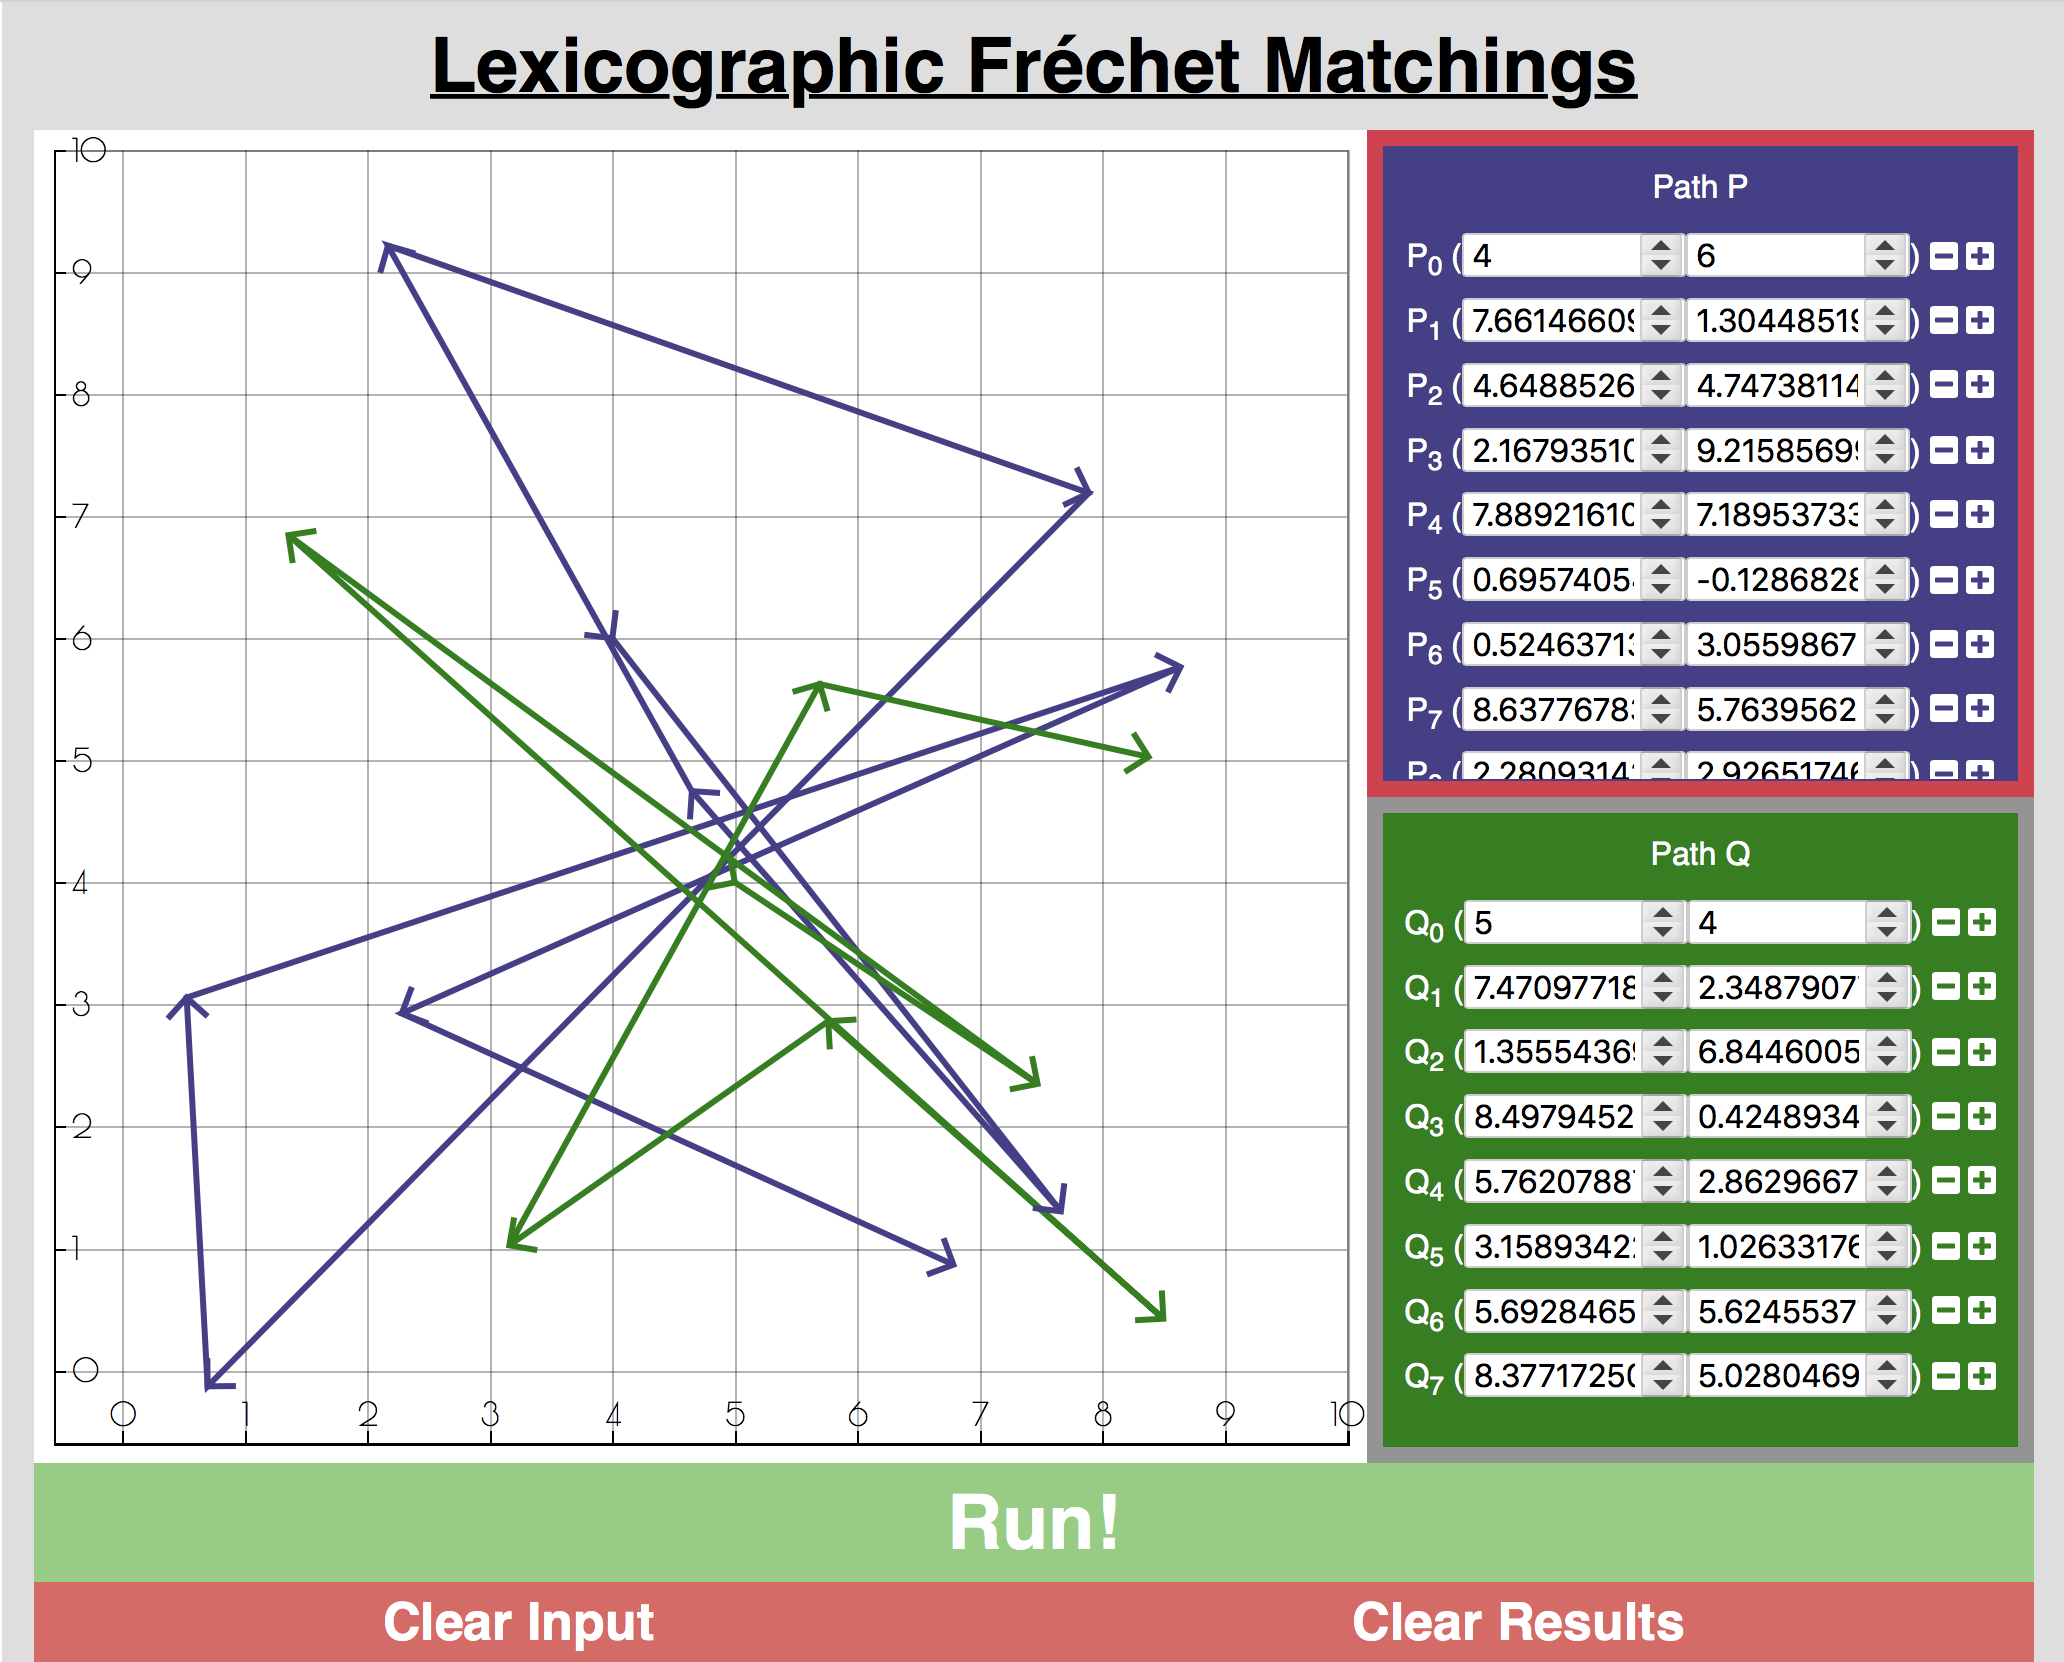
\includegraphics[width=0.8\textwidth]{webapp_input.png}
	\end{figure}
	
	\item Press ``Run". The backend executes the algorithms and the frontend visualises the results.

	\item If necessary select or deselect options like showing the free-space diagram, 
	
	\begin{figure}[H]
		\centering
		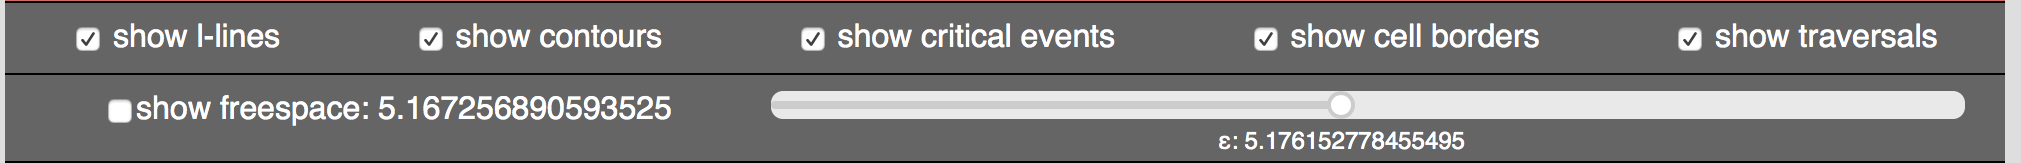
\includegraphics[width=1.0\textwidth]{webapp_options.png}
	\end{figure}
	
	\item View the height diagram $\delta$ as a contour map with critical events and traversals overlaid.
	
	
	\begin{figure}[H]
		\centering
		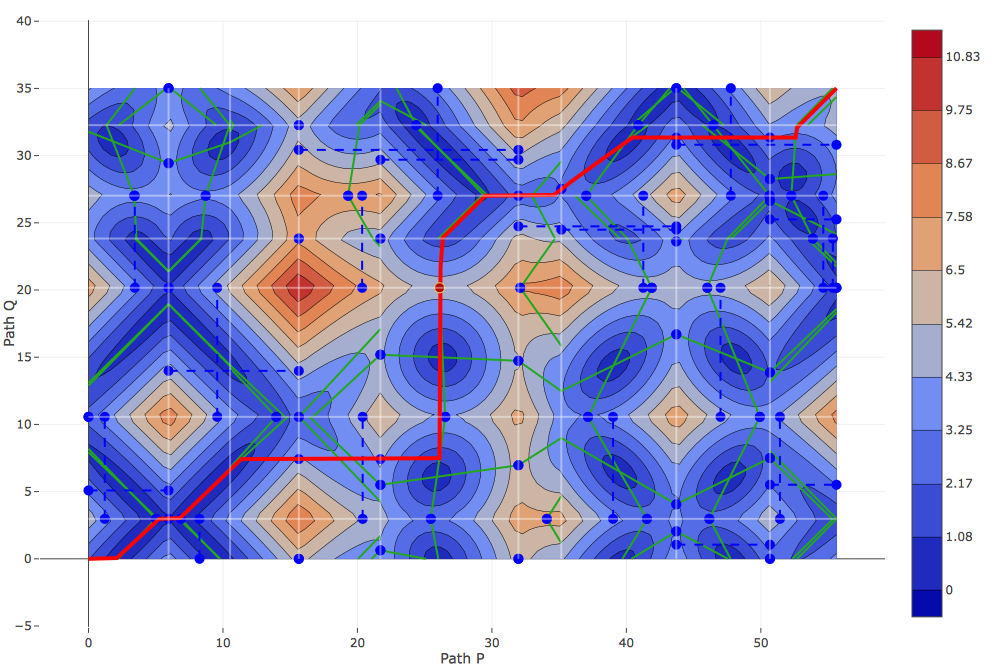
\includegraphics[width=0.7\textwidth]{webapp_2d.png}
	\end{figure}
	
	\item View the height diagram $\delta$ as a 3D model with critical events and traversals overlaid.
	
	\begin{figure}[H]
		\centering
		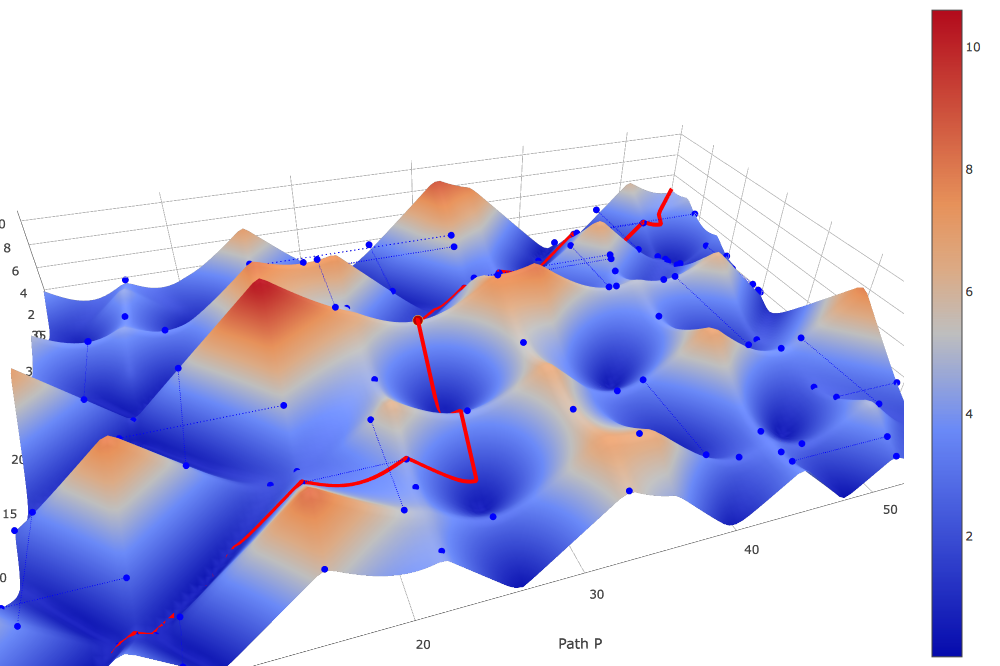
\includegraphics[width=0.7\textwidth]{webapp_3d.png}
	\end{figure}
	
	\item View the cross-sections and profiles of traversals.
	
	\begin{figure}[H]
		\centering
		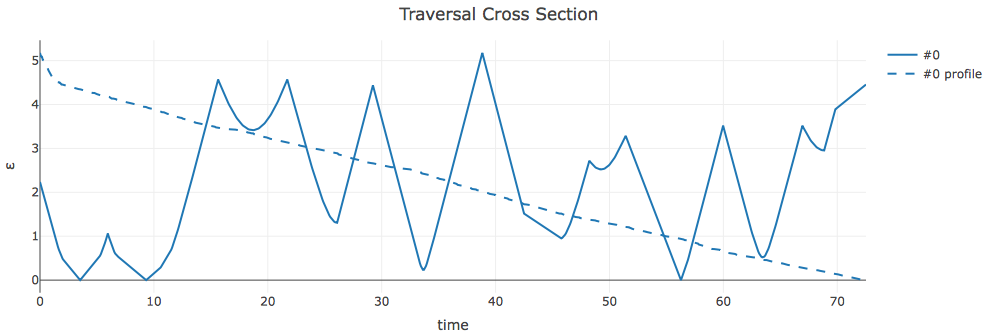
\includegraphics[width=0.7\textwidth]{webapp_cps.png}
	\end{figure}
	
	
	
\end{enumerate}


